\chapter{Bitácora 2} \label{bitacora2}
Las sugerencias y correcciones de la Bitácora 1 se detallan en los Apéndices [\ref{Apendices}], mientras que los cambios fueron realizados propiamente en la Bitácora 1 [\ref{bitacora1}]. 

\section{Parte de planificación}

\subsection{Ordenamiento de la literatura}

\begin{table}[!ht]
    \centering
    \begin{tabular}{
    | >{\centering\arraybackslash}m{2.5cm} | >{\centering\arraybackslash}m{2.7cm} | >{\centering\arraybackslash}m{3cm} | >{\centering\arraybackslash}m{3cm} | >{\centering\arraybackslash}m{1cm} | >{\centering\arraybackslash}m{2.5cm} |
    }
    \hline
    \multicolumn{3}{|c|}{\textbf{Organización}} & \multicolumn{3}{c|}{\textbf{Literatura}} \\
    \hline
    \textbf{Tipo} & \textbf{Tema General} & \textbf{Tema Específico}& \textbf{Título} & \textbf{Año} & \textbf{Autor(es)} \\ 
    \hline
    Metodológica & Correlación y Análisis de datos & Relevancia del Índice de felicidad & Crecimiento económico, progreso social y felicidad & 2017 & Luisa Montuschi \\ \hline
    Metodológica & Correlación y Análisis de datos & Relación felicidad-salud & Salud y Felicidad en Uruguay & 2010 & Mariana Gerstenblüth, Todd Jewell y Máximo Rossi \\ \hline
    Metodológica & Correlación y Análisis de datos &  Relación felicidad-progreso & ¿Suponen las directrices politicoeconómicas del Reino de Bután,... & 2014, 2015 & Ignacio Aguilar, Oriol-Jordi Andrés, Guillem Foucault, et al. \\ \hline        Metodológica & Correlación y Análisis de datos & Relación movilidad social-felicidad & Movilidad social, preferencias redistributivas y felicidad en Colombia. & 2011 & Juliana Londoño Vélez \\ \hline
    \end{tabular}
\end{table}

\newpage
\section{Enlaces de la literatura}

En el siglo XXI, se ha cuestionado la capacidad del Producto Interno Bruto (PIB) para medir adecuadamente el progreso social, dando lugar al desarrollo de nuevos indicadores como el Índice de Progreso Social y el Índice de Felicidad Nacional Bruta. Estos indicadores emergentes buscan superar las limitaciones del PIB al abordar aspectos más amplios del bienestar y la felicidad de la sociedad. La organización Social Progress Imperative ha liderado esfuerzos para crear el Social Progress Index, mientras que el Gross National Happiness Index, publicado anualmente desde 2012 en el World Happiness Report, también ha ganado reconocimiento.\\

\textbf{Resumen:} Lograr que el Producto Interno Bruto (PIB) mida correctamente el progreso social es un gran cuestionamiento ante la relevancia del índice con la realidad vivida por la sociedad. En un país centrado en el progreso, es importante abarcar todo lo posible sobre la realidad humana,  lograr cuantificarlo, y así dando un mejor resultado en el futuro. Por ello, se han creado varios índices sociales, como el Social Progress Index y el Gross National Happiness Index para lograr comparar e inclusive superar las limitaciones de los índices de progreso económico, como tiene el Producto Interno Bruto, y así no solo tomar en cuenta un progreso económico que puede ser muy centralizado, si no observar un muestreo de la realidad de las personas con características sociales. \\

\textbf{Contraste:} Por otro lado, últimamente se han dado varios eventos catastróficos, uno de estos es la pandemia del Covid-19, que han hecho a los países contemplar aun más la situación de sus habitantes. En sí, ``La pandemia puso al descubierto la vulnerabilidad de las sociedades y resaltó la interconexión entre factores sociales, naturales y económicos.'' (Alkire, 2023). Poner en alarma a la población de los países hace analizar datos vitales como los de este estudio.\\

\textbf{Contribución propia:} La reflexión sobre la necesidad de ir más allá del Producto Interno Bruto (PIB) para medir el progreso social es crucial en un mundo de constante cambio y enfrentando desafíos globales como lo fue la pandemia del Covid-19. La crisis sanitaria ha puesto resaltado la importancia de considerar no solo los aspectos económicos, sino también los sociales, para comprender verdaderamente el bienestar de las sociedades. \\

El estudio analiza la relación que existe entre el estado de salud y felicidad auto percibida, en el territorio de Uruguay a lo largo del año 2008. Se asocia el hecho de gozar de un buen estado de salud con un nivel mas alto de felicidad, siendo este a su vez, uno de los mayores determinantes de la felicidad. Se realiza un estudio además de diversas variables como lo son: desempleo, completación de la educación terciaria, religiosidad, así como factores socioeconomicos con la felicidad. Se estudia la influencia que puede representar la endogeneidad para encontrar una relación con respecto a la felicidad. Finalmente, se concluye con la importancia que representa el estado de salud con respecto a la felicidad en Uruguay. \\

En el caso de Uruguay, el estudio busca concentrar la investigación entre la relación que se desarrolla entre la felicidad personal y la auto-percepción del estado de salud, utilizando la encuesta Religión, Salud y Emancipación Juvenil del ISSP para Uruguay en el 2008. Del estudio se obtiene que la salud es la variable que presenta la mayor relación con respecto a la felicidad. Para evitar problemas de heterogeneidad observable que se pueda desarrollar en dicha variable, se realizan estimaciones utilizando métodos pertinentes. Estos resultados se ven respaldados por estudios realizados en la misma región con anterioridad obteniendo resultados similares\\

\textbf{Resumen:} La investigación busca encontrar la relación existente entre la salud y la felicidad en Uruguay, se trata como variable dependiente a la felicidad, la cual se observa como una variable binaria, en la cual el individuo se reporta como feliz o no. Debido a la dificultad que presentan los problemas de endogeneidad se busca utilizar métodos adecuados para establecer las relaciones, uno de los utilizados es el \textit{propensity score}, lo cual busca un control de variables socioeconómicos para estimar el efecto que presenta la salud directamente en la felicidad, además de utilizarse métodos de relación como \textit{nearest neighbors}, Kernel y estratificación, así como \textit{Average Treatment effect on the Treated}. De forma resumida, el estudio busca la relación que existe entre diversos factores, enfocados en la salud, con respecto a la felicidad y a su vez utilizando métodos para reducir los posibles sesgos debido a la naturaleza de los datos.\\

\textbf{Contraste:} De la misma forma que concluye Amado Peiró (2001) en Condiciones Socioeconomicas y Felicidad de los Españoles, la salud resulta ser un factor sumamente importante para determinar la felicidad, la relación que presenta resulta intuitiva y corresponde de forma positiva con una multitud de estudios realizados con anterioridad, mientras que otras variables presentan una relación menor o casi inexistente, la salud se observa con una relación fundamental con respecto a la felicidad, ya sea en territorios de América Latina, como se expone en el estudio de Gerstenbluth, así como en territorios Europeos.\\

\textbf{Contribución propia: }Se observa en base a las relaciones obtenidas tanto en España como en Uruguay que la salud sobresale como un factor crítico para determinar la felicidad personal. Se observa que el bienestar físico y mental están fuertemente relacionados con la felicidad. Ambos estudios buscan tratar de forma adecuada los problemas de endogeneidad y sesgos en la estimación de efectos causales, para esto se utilizan métodos como el \textit{propensity score} y técnicas de correspondencia. La evidencia del análisis posterior demuestra la relevancia que presenta la salud como uno de los determinantes más importantes de la felicidad en distintos contextos territoriales. Políticas y programas impulsados por el gobierno tienen el potencial de generar un impacto significativo en la felicidad de las distintas poblaciones, los resultados pueden ser de interés para el diseño de políticas públicas y estrategias gubernamentales.\\

Bután tuvo un crecimiento económico bastante significativo entre los años 1980-2013, espacio en que se realiza el análisis. Esta economía se destaca entre sus vecinos, inclusive teniendo el segundo crecimiento más alto en todo el mundo por un momento. Además, la Felicidad Interna Bruta (FIB) de Bután también destaca. La investigación intenta hacer una correlación entre las variables para intentar postular a la economía dada como ejemplar, y dado esto logra intuir que, por ejemplo, una gran riqueza no implica una felicidad más grande. El estudio compara con Nepal, Bangladesh, en métodos cercanos porque son economías similares, y también con economías grandes, donde se logra ver que Bután se comporta en correlación de manera distinta al mundo, donde entre más crecimiento económico se logre, más alto es el Índice de Felicidad.\\

\textbf{Resumen:} El estudio comienza intentando enfatizar la relevancia de la felicidad, en especial en el caso específico de Bután. Denota que la orientación popular es concentrarse en el Producto Interno Bruto, indicador del progreso económico muy central en los países, cuando dejan de lado lo que puede ser la felicidad de la sociedad. Dentro del estudio se logra ver algunos índices de diferentes países para poder contrastarlo con el caso de Bután. Dentro de este, se utilizan diferentes gráficos y correlaciones para lograr distinguir los diferentes países, así igual de manera conjunta, donde se exponen varios países y el mundo. La investigación trata comprender la correlación positiva de Bután entre los indicadores del Producto Interno Bruto y la Felicidad Interna Bruta, y lo compara con el resto del mundo, viendo cierto patrón a tener una correlación negativa. También trae al caso a Nepal y Bangladesh, para tratar de hacer la comparación más cercana. Sus gráficos y análisis le permite hacer la conclusión de que, aunque significativo progreso económico en los países en las últimas décadas, no se ha visto la misma fuerza en la felicidad, e intenta enfocar que se debería seguir como marco de ejemplo el caso de Bután. \\

\textbf{Contraste:} Sin embargo, como lo trabaja Abraham Aparicio Cabrera (2019) con \textit{Economía y Felicidad}, la economía de la felicidad es una rama importante de la economía, proponiendo el ingreso y consumo como variables relevantes y bases del bienestar general de las personas. ``Aunque la economía de la felicidad es un campo muy activo en las últimas tres décadas, algunos autores creen que es exagerado hablar de una disciplina subalterna de la economía'', en especial si estamos tratando de relacionar ambas variables principales por fuera del marco teórico, sino del práctico. Aparicio procede a encontrar diferentes percepciones de la felicidad, y subdividirlas, entre sacrificio y esfuerzo, con placer y dinero; que podemos observar como la satisfacción social y económica. Si bien es cierto que la felicidad cuenta con gran relevancia de la felicidad al menos subjetivamente, este estudio enfoca que hay una leve división en la relación de las variables. \\

\textbf{Contribución propia:} El caso de Bután es bastante particular ya que no sigue el patrón mundial, mostrando ambos indicadores de progreso económico y felicidad subir conjuntamente. Si bien es cierto que el muestreo son pocos años para llegar a una conclusión certera, al menos en el corto plazo se logra distinguir que el resto del mundo no sigue la misma línea que Bután. La subjetividad de la felicidad es bastante relevante también en casos de estudio como estos, pues los datos pueden estar sesgados localmente ante un concepto de felicidad percibido, donde por ejemplo un país desarrollado intenta de buscar un progreso social mientras la felicidad en otros países más bien yace en poder organizar bien los materiales económicos. Por eso tratar con temas como la economía de la felicidad y la leve división de la felicidad como diferentes percepciones es crucial para el comprendimiento de una satisfacción social \\

El estudio busca relacionar los determinantes de ingreso, movilidad social e injusticia social con el nivel de felicidad de sus habitantes, tratando de hacer un empate entre los resultados empíricos del estudio con las observaciones teóricas que han tenido otros contemporáneos. El estudio logra el objetivo de validar algunas observaciones teóricas, pero contradiciendo otras, además de encontrar que el nivel de ingreso si motiva a la felicidad, pero que no influye en las políticas de redistribución de la riqueza. \\

\textbf{Resumen:} El estudio de Londoño buscaba buscar una relación entre los determinantes de movilidad social, ingreso y justicia social con la felicidad y la demanda de redistribución. Donde las conclusiones finales de este estudio se pueden resumir en tres puntos, el primero es que las personas del estudio resultaron ser pesimistas en cuanto a su experiencia en la movilidad, pero que tenían buenas perspectivas de sus hijos para que ellos si tuvieran más movilidad social. Luego el otro hallazgo es que las personas de mayor ingreso tienen más felicidad que las personas de menor ingreso. Y como último punto, el ingreso resulta ser un determinante pobre de la demanda de redistribución, es decir, que no necesariamente las personas de ingresos más altos quieren una economía libre. \\

\textbf{Contraste:} El trabajo hace un desarrollo exhaustivo por dejar claro qué son todas las variables que va a tomar en cuenta, también indica la importancia que tiene una buena definición de felicidad para poder tratarla desde un punto de vista económico, ya que se llega a la conclusión de que aunque hay relación positiva ingreso-felicidad, sigue siendo muy débil y que tratar un concepto tan amplio como la felicidad desde una rama del conocimiento no es lo óptimo, pues al ser un concepto tan grande, necesita que haya un trabajo interdisciplinario para poder abordarla con mayor detalle y precisión. \\

\textbf{Contribución propia:} Como podemos observar ambos estudios tiene un enfoque de determinar si la felicidad se ve afectada por ciertos factores, en este caso, uno que tienen en común es el ingreso y hacen buenas acotaciones extras de ciertos resultados. Para llevar un orden, ambos estudios comienzan el análisis definiendo qué se entiende por felicidad, cómo se analiza y desde qué punto de vista lo harán, aunque ambos estudios lo hacen desde el punto de vista económico, dejan muy en claro al lector que este concepto va más allá de un punto de vista económico, pues es un término que ha intentado ser definido desde la filosofía y psicología, hasta últimamente en la economía. \\

Ambos estudios suponen que la felicidad viene dada por una utilidad, y bien ambas mencionan que esta es una falencia que tienen ambos estudios, pues hay otros factores que afectan enormemente a la felicidad, como lo son la cultura de país, por ejemplo. Luego cada uno va a utilizar una metodología diferente, donde el estudio de Londoño se hace una revisión bibliográfica, análisis de datos y un trabajo de campo para poder tener más información, el estudio de Álvarez lo hace desde una fuerte revisión bibliográfica y análisis de datos, sin presentar un trabajo de campo, sin embargo, en el estado del arte de cada uno de estos trabajos, hay muchas referencias donde tienen estudios con otro tipo de metodologías y que al final llegan a conclusiones igual o muy similares, lo que hace que se refuercen entre ellas y agregando información adicional, que también refuerza, en el estudio actual respectivo. \\

Antes de seguir, es importante mencionar la paradoja de Easterlin, quien fue pionero en definir la felicidad desde el punto de vista económico, haciendo uso de la función de utilidad para ello. Esta paradoja indica que, a mayores niveles de ingreso menor es el aumento en la felicidad, lo que es lo mismo que hay una Utilidad Marginal Decreciente. Ambos estudios parten de esta idea, pues nace la pregunta ¿Qué tanto impacto hay dado tales factores? Tanto el estudio de Londoño, como el estudio de Álvarez llegan a la conclusión de que hay una relación positiva entre ingreso y felicidad de las personas, aunque también hacen el hincapié de que esta relación es muy débil, pues estamos delimitando el concepto de felicidad a una sola área que vendría siendo la económica.\\



\newpage

\subsection{Fichas nuevas de literatura}
\begin{table}[!ht]
    \caption{Ficha de Literatura 5}
    \begin{center}
        \begin{tabular}{  m{3cm} | m{12cm}  }
        \hline\textbf{ Encabezado} & \textbf{Contenido }\\ \hline
        Título: & Economía de la felicidad: Incidencia de los cambios de las variables macroeconómicas sobre la felicidad de los habitantes de américa latina. \\ \hline
        Autor(es): & Daniela Álvarez Zuluaga \& Caroline Londoño Díez  \\ \hline
        Año: & 2016 \\ \hline
        Nombre del tema: & Relación entre felicidad, ingreso, PIB, ICTR y Balanza Comercial. \\ \hline
        Cronológica: &  2003-2016 \\ \hline
        Metodológica: & Metodología de carácter cuantitativo y va a ser desarrollada a través de un modelo de panel de datos, el cual será de tipo estático. \\ \hline
        Temática: & Estudios económicos y psicológicos \\  \hline
        Teórica: & Economía de la felicidad. \\ \hline
        Resumen en una oración: & Qué factor afecta más a la felicidad dado el PIB, inflación, ITCR y BC. \\ \hline
        Argumento central: &  Determinar cómo los factores mencionados afectan a la felicidad \\ \hline
        Problemas con el argumento o el tema: & No toma en cuenta el desempleo que sería un factor muy considerable a tener en cuenta. Además, es un estudio de análisis y revisión bibliográfica, no hubo trabajo de campo, porque está tratando con datos anteriores e información que posiblemente ya ha cambiado. \\ \hline
        Resumen en un párrafo: & El ensayo hace un trabajo exhaustivo por dejar claro qué son todas las variables que va a tomar en cuenta, también indica la importancia que tiene una buena definición de felicidad para poder tratarla desde un punto de vista económico, ya que se llega a la conclusión de que aunque hay relación positiva ingreso-felicidad, sigue siendo muy débil y que tratar un concepto tan amplio como la felicidad desde una rama del conocimiento no es lo óptimo, pues al ser un concepto tan grande, necesita que haya un trabajo interdisciplinario para poder abordarla con mayor detalle y precisión. \\ \hline
        \end{tabular}
    \end{center}
\end{table}

\begin{table}[H]
    \caption{Ficha de Literatura 6}
    \begin{center}
        \begin{tabular}{  m{3cm} | m{12cm}  }
        \hline\textbf{ Encabezado} & \textbf{Contenido }\\ \hline
        Título: &  Economía y felicidad: ¿Importa lo que las personas entienden por felicidad?\\ \hline
        Autor(es): & Abraham Aparicio Cabrera \\ \hline
        Año: &  2019\\ \hline
        Nombre del tema: & Conexión entre la felicidad y la economía \\ \hline
        Cronológica: & 2014 \\ \hline
        Metodológica: & Estudio de bases de datos de una encuesta. Contrastes, comparaciones y correlaciones  \\ \hline
        Temática: & Estudios económicos y psicológicos\\ \hline
        Teórica:  & Economía de la felicidad \\ \hline
        Resumen en una oración: & Los factores económicos son vitales a la hora de percibir la felicidad según las personas \\ \hline
        Argumento central: & Averiguar la relación entre la percepción de felicidad y los factores económicos \\ \hline
        Problemas con el argumento o el tema: & Como recalca el artículo, la felicidad puede ser algo subjetivo y difícil de cuantificar, en términos relativos con el progreso económico. Además, la muestra parece un poco localizada, por lo que los datos podrían estar sesgados a una sección local.  \\ \hline
        Resumen en un párrafo: & El estudio define por un lado la felicidad y la economía de la felicidad. Hace uso de una base de datos basada en la Encuesta Nacional de Satisfacción con la Vida y la Sociedad, creada por la Universidad Nacional Autónoma de México. En este, encuentra varias conexiones y datos que destacan en las creencias populares de las personas, pero solo se visualizan porcentajes y no muestras agrupadas, como para poder comparar los grupos varios de diferentes ingresos. También destaca la felicidad como placer y dinero, o la felicidad como sacrificio y esfuerzo, al lograr encontrar grandes cantidades de observaciones que se inclinaban a alguna de las dos.   \\ \hline
        \end{tabular}
    \end{center}
\end{table}

\begin{table}[H]
    \caption{Ficha de Literatura 7}
    \begin{center}
        \begin{tabular}{  m{3cm} | m{12cm}  }
        \hline\textbf{ Encabezado} & \textbf{Contenido }\\ \hline
        Título: &  Condiciones Socioeconomicas y
        Felicidad de los Españoles
        \\ \hline
        Autor(es): & Amado Peiró \\ \hline
        Año: &  2001\\ \hline
        Nombre del tema: & Conexión entre la felicidad y condiciones socioeconomicas \\ \hline
        Cronológica: & 1995 \\ \hline
        Metodológica: & Estudio de bases de dato de una encuesta. Contrastes, comparaciones y correlaciones  \\ \hline
        Temática: & Estudios económicos y psicológicos\\ \hline
        Teórica:  & Economía de la felicidad \\ \hline
        Resumen en una oración: & Encontrar una aproximación de la relación entre condiciones socio económicas y felicidad desde la evidencia disponible en España. \\ \hline
        Argumento central: & Impacto de las condiciones socio económicas con respecto a la felicidad desde la evidencia disponible en España\\ \hline
        Problemas con el argumento o el tema: & El estudio establece la felicidad como una variable compleja que requiere un acercamiento no únicamente desde un punto de vista económico, sino que la observa como una variable compleja que requiere un estudio tanto psicológico como sociológico  \\ \hline
        Resumen en un párrafo: & Inicialmente se describen las limitaciones presentes del estudio de la felicidad al tratarse de una variable compleja con elementos no únicamente económicos sino psicológicos y sociológicos. Seguido de esto se procede a explicar la base de datos a estudiar, la cual corresponde a los obtenidos de la Encuesta Mundial de Valores, misma que se realizó en España en 1995. Se establecen los principales factores ligados a la felicidad, estableciendo relaciones bivariadas con respecto a la felicidad, además se establecen tablas adecuadas acerca de las relaciones encontradas. Finalmente se reporta los hallazgos encontrados, se concluye que tanto la salud como la edad representan una fuerte relación con la felicidad de los individuos. \\ \hline
        \end{tabular}
    \end{center}
\end{table}

\begin{table}[H]
    \caption{Ficha de Literatura 8}
    \begin{center}
        \begin{tabular}{  m{3cm} | m{12cm}  }
        \hline\textbf{ Encabezado} & \textbf{Contenido }\\ \hline
        Título: &  Lecture Notes on Asymptotic Statistics \\ \hline
        Autor(es): & Changliang Zou \\ \hline
        Año: &  2014\\ \hline
        Nombre del tema: &  Transformaciones de estadísticos: El método Delta\\ \hline
        Cronológica: &  N.A. \\ \hline
        Metodológica: & Método Delta \\  \hline
        Teórica: &  Transformaciones de estadísticos\\ \hline
        Resumen en una oración: &  Aplicaciones del método delta para obtener la distribución de las transformaciones de estadísticos. \\ \hline
        Argumento central: &  Lo esencial de este documento es el ejemplo 2.4.2. ya que sirve de guía para unir la correlación con la aproximación de la distribución de una variable. \\ \hline
        Problemas con el argumento o el tema: &  De momento no se puede determinar de manera concreta los problemas con el argumento ya que únicamente se está estableciendo la base de la idea a seguir. En el peor de los casos, el peor problema sería que no funcione para lo que se espera.\\ \hline
        Resumen en un párrafo: & Este documento con alta rigurosidad matemática se puede ver como una guía con metodologías estadísticas que se pueden llevar a cabo para diferentes aplicaciones. De momento nos vamos a enfocar en la sección con la información del método delta, el cual nos permitirá aproximar la distribución de dado parámetro, por medio de aplicaciones que se le pueden realizar a las transformaciones de los estadísticos.\\ \hline
        \end{tabular}
    \end{center}
\end{table}

\newpage

\section{Análisis estadísticos}
El proyecto se está desarrollando en el repositorio de \textbf{\href{https://github.com/bluke7ide/Proyecto_Estadistica}{GitHub}}, [\ref{github}] por si se desea ver completo.
\subsection{Análisis descriptivo}

Para las bases de datos a utilizar se decide reemplazar los valores N/A presentes en distintas entradas por el promedio de la variable en cuestión. La existencia de valores N/A es debido a que no todos los países reportan todos los años a las tres entidades de las cuales se obtienen los datos, esto a raíz de las distintas dinámicas geo-socio-políticas que se desarrollan en las divisiones geográficas del mundo, así como la calidad de las relaciones que existe entre los países, situaciones de guerra o crisis. \\

En la estructura que presentan los datos se puede observar que cada variable tiene una columna propia; no existe una combinación de distintas variables en la misma columna o alteraciones de variables. A su vez, cada observación es única, puesto que se trata de un país por observación, y sus valores están distribuidos a lo largo de una única fila. Debido a la estructura que traía la base de datos, no fue necesario el uso de funciones como pivot\_longer o pivot\_wider. \\

Así mismo, existe un identificador claro para cada una de las entradas, en este caso corresponde a la columna \textit{country} que indica el país, como lo dicho anteriormente. Por otro lado, queremos que todas las variables manejen valores numéricos, así que se va a reemplazar los valores de \textit{income\_class} por su factor, para de esta forma tener únicamente variables numéricas, y para efectos de análisis de correlación, la variable ``country'' no toma gran peso, entonces se decide dejar de lado.\\

Al cumplirse las características anteriores podemos asegurar que la forma actual que presentan los datos se encuentran de la forma ``tidy''. De esta forma, la tabla se encuentra lista para realizar el análisis de datos exploratorio descriptivo.\\

Para comenzar, lo que vamos a realizar es un análisis descriptivo completo de la tabla. La forma más sencilla de empezar este proceso es mediante la función ``descr'', la cual permite obtener distintos estadísticos de la tabla en cuestión. Se procede a utilizar dicha función y se obtiene la tabla siguiente. Se decide obtener los datos relevantes de esta tabla para facilitar la lectura. 

\pagebreak

\begin{table}[!ht]
\caption{Estadísticas descriptivas de la base de datos}
    \centering
    \begin{tabular}{l|*{7}{>{\raggedleft\arraybackslash}p{1cm}}}
        \hline
         Variables & Media & Desv.Est & Mín & Q1 & Mediana & Q3 & Máx \\ 
        \hline
        adult\_literacy & 81 & 16 & 24 & 81 & 82 & 94 & 100 \\ 
        air\_pollution & 89 & 27 & 0 & 98 & 100 & 100 & 100 \\ 
        alcohol\_consumption & 6 & 4 & 0 & 2 & 5 & 9 & 17 \\ 
        cpi & 43 & 20 & 9 & 30 & 38 & 57 & 89 \\ 
        electricity\_access & 83 & 27 & 5 & 75 & 100 & 100 & 100 \\ 
        freedom\_to\_make\_life\_choices & 1 & 0 & 0 & 1 & 1 & 1 & 1 \\
        gdp (en billones) & 519 & 1962 & 1 & 15 & 549 & 320 & 19228 \\ 
        gdp\_capita (en miles) & 14 & 20 & 0,3 & 2 & 5 & 17 & 111 \\ 
        generosity & 0 & 0 & 0 & 0 & 0 & 0 & 1 \\ 
        healthy\_life\_expectancy\_at\_birth & 63 & 7 & 43 & 59 & 65 & 68 & 74 \\ 
        income\_class & 2 & 1 & 0 & 1 & 2 & 3 & 3 \\ 
        labor\_force (en millones) & 22 & 77 & 0,2 & 2 & 4 & 13 & 779 \\ 
        labor\_rate & 61 & 10 & 34 & 55 & 61 & 66 & 87 \\ 
        land\_area (en miles) & 831 & 2077 & 0,3 & 54 & 215 & 652 & 16377 \\
        life\_expectancy & 72 & 8 & 52 & 66 & 74 & 79 & 84 \\ 
        life\_ladder & 5 & 1 & 3 & 5 & 5 & 6 & 8 \\ 
        log\_gdp\_per\_capita & 9 & 1 & 7 & 8 & 9 & 10 & 12 \\
        negative\_affect & 0 & 0 & 0 & 0 & 0 & 0 & 1 \\ 
        perceptions\_of\_corruption & 1 & 0 & 0 & 1 & 1 & 1 & 1 \\ 
        population (en millones) & 49 & 164 & 0,3 & 5 & 11 & 34 & 1392 \\
        population\_density & 212 & 691 & 2 & 34 & 81 & 187 & 7874 \\ 
        positive\_affect & 1 & 0 & 0 & 1 & 1 & 1 & 1 \\ 
        social\_support & 1 & 0 & 0 & 1 & 1 & 1 & 1 \\ 
        unemployment\_rate & 7 & 5 & 0 & 4 & 6 & 10 & 24 \\ 
        water\_access & 87 & 16 & 41 & 80 & 94 & 99 & 100 \\ \hline
    \end{tabular}
\end{table}

\begin{quote}
    \textit{Fuente: Elaboración propia a partir de las base de datos de The World Bank (2018), Transparency International (2018) y World Happiness Report (2018)}\\
\end{quote}


Una vez obtenidos los estadísticos descriptivos de cada variable, tenemos indicadores claros de su comportamiento, pero para el estudio que se desea desarrollar es necesario obtener a su vez, la forma en la que se relacionan las distintas variables entre ellas. Por lo que resulta sensato el obtener una matriz de correlación entre las distintas variables para tener índices normalizados que muestren la forma en la cual se comporta una variable con respecto a otra, pero la gran cantidad de variables presentes en la base de datos dificulta que se aprecie de forma adecuada la matriz, por lo que se utiliza un gráfico de correlación entre las variables.

\pagebreak

\begin{figure}[!ht]
    \centering
    \caption{Gráfico de correlaciones}
    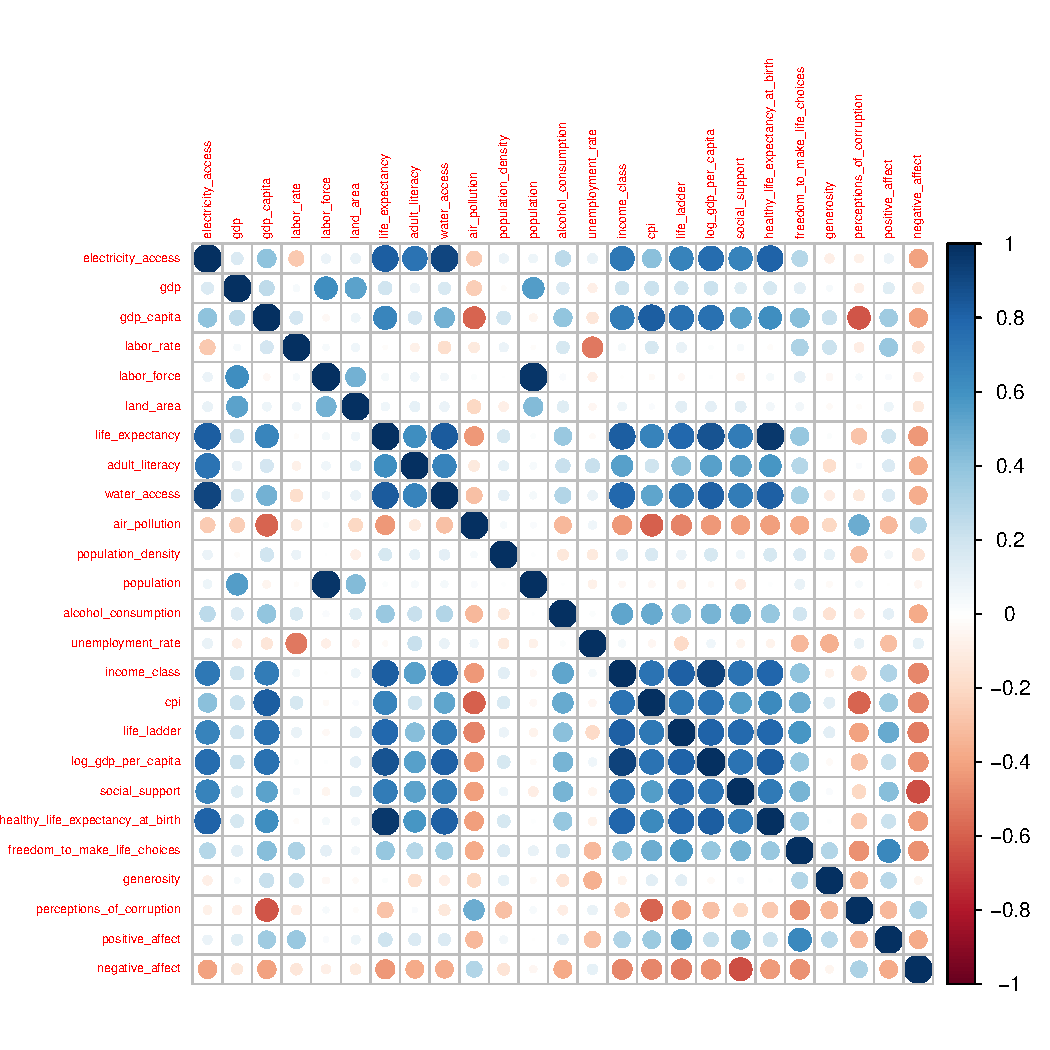
\includegraphics[width=0.9\textwidth]{figures/correlaciones.pdf}
    \label{fig:correlaciones}
\end{figure}

Del gráfico de correlación se logra observar de forma sencilla cuáles son las variables que tienen una relación más fuerte con nuestra variable de estudio, \textit{life\_ladder}. Estas corresponden a \textit{electricity\_access, gdp\_capita, life\_expectancy, water\_access, income\_class, cpi, log\_gdp\_per\_capita, social\_support, healthy\_life\_expectancy\_at\_birth,} y \textit{freedom\_to\_make\_life\_choices.}

\newpage

Hacer énfasis que \textit{life\_ladder} es nuestro Índice de Felicidad, conformado por el promedio de las respuestas a una encuesta sobre felicidad, donde se les preguntaba a las personas que ubicaran su vida del 0 al 10, siendo 0 el peor de los casos y 10 el mejor. , el presente estudio busca relacionar variables del progreso socioeconómico del país con respecto a \textit{life\_ladder}, nuestra variable de interés. Por ello se decide tomar como variables relevantes las siguientes:

\begin{itemize}
    \item \textit{electricity\_access}: El acceso de la población a la electricidad se observa como un factor importante en la promoción de la educación y la información, lo que tienen repercusión en la productividad de un territorio en especifico, además de que un índice mayor, representa el acceso en zonas rurales, lo cual se observa como catalizador de desarrollo económico.
    \item \textit{water\_access}: El acceso de la población al agua potable se presente como factor fundamental en salud y bienestar, para ser mas específicos en seguridad alimentaria, lo cual es un factor fundamental no solo para el desarrollo económico sino para el funcionamiento integral de cualquier sociedad.
    \item \textit{income\_class}: La clase social dominante está estrechamente ligada con respecto al progreso económico del país, pues una clase económica de un estrato superior esta relacionada con países primer mundistas, los cuales tienen un progreso económico mucho mayor al resto del mundo.
    \item cpi: El índice de percepción de corrupción tiene una fuerte relación con los gobiernos de turno de las distintas naciones, los cuales tienen gran influencia en los mercados y permisos para el desarrollo económico presente en los países. Esta percepción de corrupción no sólo identifica a los países, pero los condiciona en tratados o comercios con otros países. 
    \item \textit{log\_gdp\_per\_capita}: El PIB per capita ha sido uno de los factores más determinantes en el desarrollo económico, así como uno de los más utilizados debido a su relación significativa con la economía de un país. Se decidió utilizar la forma logarítmica de este, debido a que el Producto Interno Bruto normal presentaba valores de magnitudes exageradas en comparación a los valores presentes en las otras variables, entonces resulta más sensato trabajar con la versión logarítmica.
\end{itemize}

 Ahora bien, se decide agregar la tabla de estadísticas descriptivas de \textit{life\_ladder}, debido a que se trata de la variable de estudio a la que queremos darle énfasis, para así poder ver las propiedades de ésta dados los datos que se utilizarán para el estudio. Al mismo tiempo, se agregan las estadísticas descriptivas de \textit{log\_gdp\_per\_capita} debido a que en la mayoría de estudios se ha utilizado el Producto Interno Bruto per-cápita como una de las variables más influyentes a la hora de analizar los factores del área económica como lo es el progreso económico. Como vimos en las referencias bibliográficas que hemos utilizado en este trabajo, estos estudios demostraron que siempre hay una correlación positiva entre ingreso, el cual casi siempre se toma como el PIB per-capita en dichos estudios en conjunto con la felicidad. \\ 

\newpage

\begin{table}[H]
    \caption{Estadísticas descriptivas combinadas}
    \centering
    \begin{tabular}{l|*{2}{>{\raggedleft\arraybackslash}p{1.5cm}}}
        \hline
        Medida & \textit{life\_ladder} & $lgpc^*$  \\
        \hline
        Mínimo & 3,08 & 6,61 \\ 
        1° Cuartil & 4,51 & 8,48 \\ 
        Mediana & 5,38 & 9,49 \\ 
        Promedio & 5,40 & 9,36 \\ 
        3° Cuartil & 6,17 & 10,29 \\ 
        Máximo & 7,69 & 11,65 \\ 
        Desv. Est. & 1,12 & 1,20 \\ 
        \hline
    \end{tabular}
\end{table}

\begin{quote}
    \textit{Fuente: Elaboración propia a partir de las base de datos de The World Bank (2018), Transparency International (2018) y World Happiness Report (2018)} 
    \footnote{$lgpc^*$: \textit{log\_gdp\_per\_capita}} \\
\end{quote}

Finalmente se agrega una tabla con estadísticas descriptivas del resto de variables, incluyendo las dos anteriores, puesto como vimos en el gráfico de correlación \ref{fig:correlaciones}, las variables que tomamos para realizar el trabajo poseen una correlación positiva. Por ende, creemos pertinente hacer una uso del análisis exploratorio de datos en estas variables, para tener más información acerca de cómo se comportan, dada nuestra base datos.\\

\begin{table}[H]
    \caption{Estadísticas descriptivas de las variables relevantes}
    \centering
    \begin{tabular}{l|*{6}{>{\raggedleft\arraybackslash}p{2cm}}}
        \hline
        Medida & \textit{ cpi} & $electric^{**}$ & \textit{income\_class} & \textit{life\_ladder} & $lgpc^*$ & \textit{water\_access} \\ \hline
        Media & 43,36 & 82,99 & 1,74 & 5,40 & 9,36 & 87,40 \\ 
        Desv.Est & 19,69 & 27,39 & 1,05 & 1,12 & 1,20 & 16,25 \\ 
        Mín & 9,25 & 5,15 & 0,00 & 3,08 & 6,61 & 40,77 \\ 
        Q1 & 29,50 & 75,31 & 1,00 & 4,51 & 8,48 & 80,16 \\ 
        Mediana & 37,50 & 99,53 & 2,00 & 5,38 & 9,49 & 94,14 \\ 
        Q3 & 56,75 & 100,00 & 3,00 & 6,18 & 10,29 & 99,32 \\ 
        Máx & 89,25 & 100,00 & 3,00 & 7,69 & 11,65 & 100,00 \\ 
        \hline
    \end{tabular}
\end{table}

\begin{quote}
    \textit{Fuente: Elaboración propia a partir de las base de datos de The World Bank (2018), Transparency International (2018) y World Happiness Report (2018)} \footnote{$electric^{**}$: \textit{electricity\_access}}
\end{quote}

\pagebreak

Dejando de lado las relaciones por un momento, nos vamos a centrar en la variable \textit{life\_ladder}. La Figura \ref{fig:life_ladder} permite tener una visualización clara acerca de la distribución que presenta esta variable, así como ser una herramienta útil para identificar la tendencia central por la cual se rigen estos datos. Algo semejante ocurre para poder los datos atípicos. Aunque se tiene una tabla con las estadísticas descriptivas de la variable, resulta mucho mas intuitivo estudiar la data de una forma visual; con la tabla de variables descriptivas junto con el gráfico del comportamiento de \textit{life\_ladder} se puede realizar un estudio completo de la variación de esta.

\begin{figure}[H]
    \centering
    \caption{Gráfico del comportamiento de \textit{life\_ladder}}
    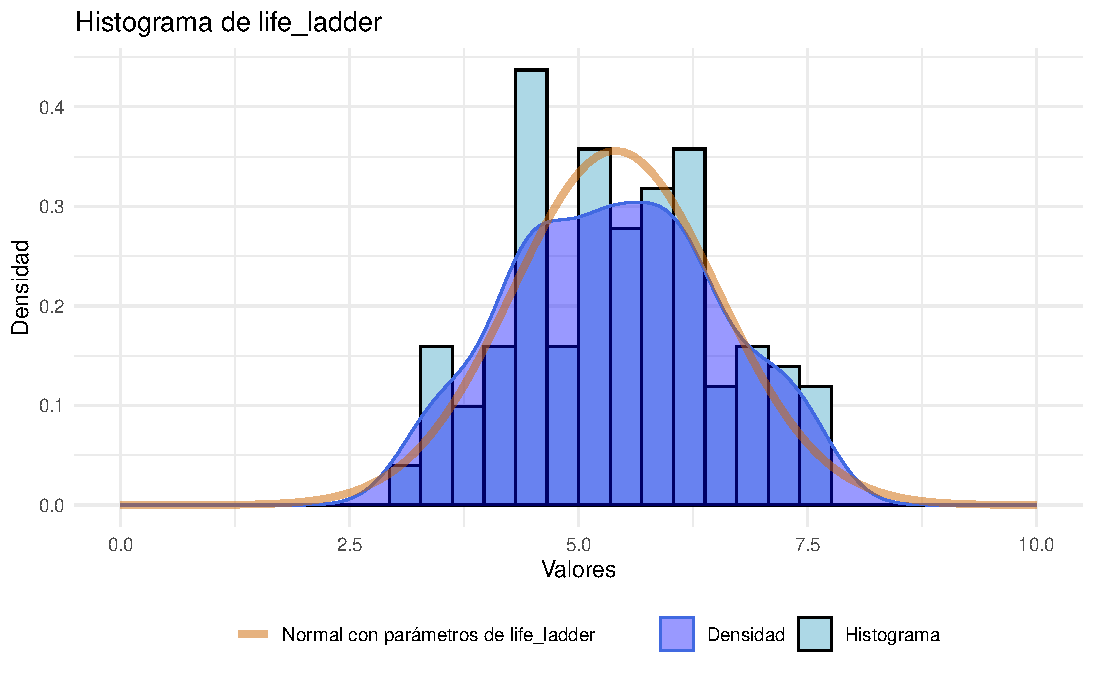
\includegraphics[width=1\textwidth]{figures/life_ladder.pdf}
    \label{fig:life_ladder}
\end{figure}

Notar que se agregó solo de referencia una distribución normal, con los parámetros que tiene \textit{life\_ladder}. De esta manera, se puede notar que la densidad de \textit{life\_ladder} es bastante similar a esta normal. Algo similar ocurre si estandarizamos \textit{life\_ladder}, aunque sería exactamente el mismo gráfico y con una distribución normal con parámetros 0 y 1. 

\pagebreak

Por otro lado, \textit{log\_gdp\_per\_capita} es una de las variables que presenta mayor relación con \textit{life\_ladder}, el gráfico de estas dos variables [\ref{fig:lgdp_life}] nos permite apreciar de forma más clara la relación positiva que existe entre estas dos, esto debido a que el Producto Interno Bruto es uno de los componentes más fundamentales para medir el progreso económico de una nación. Es por esto que obtener una relación positiva entre este y \textit{life\_ladder} resulta claro para contestar la pregunta de investigación planteada.

\begin{figure}[H]
    \centering
    \caption{Gráfico de life\_ladder relacionado con log\_gdp\_per\_capita}
    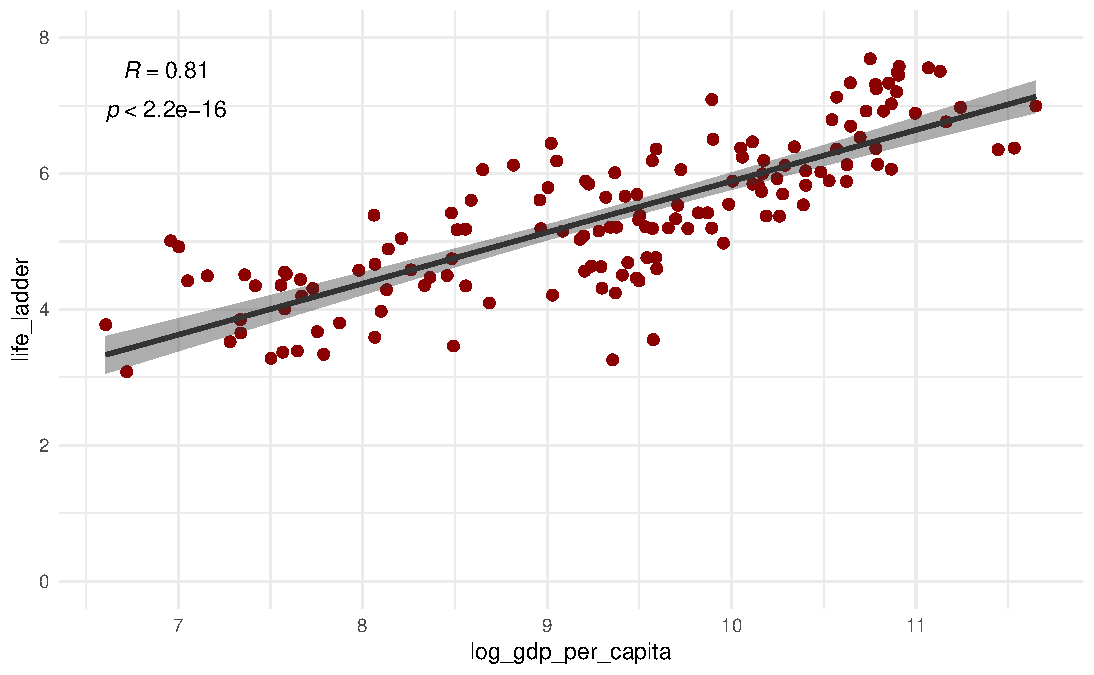
\includegraphics[width=1\textwidth]{figures/lgdp_life.pdf}
    \label{fig:lgdp_life}
\end{figure}

Notar que el coeficiente de correlación de Pearson da 0.81, una relación fuerte de las variables. Además, el valor-p mostrado corresponde a la hipótesis de que la correlación no debe de ser 0, para que tengan algún tipo de relación. Al acercarse el valor p a 0, podemos estar seguros de que si la hipótesis se acepta, entonces tiene un margen demasiado bajo de que sea verdaderamente cierta. Resulta de la misma manera si se hace la hipótesis de que la correlación debe de ser positiva, ya que la manera en que están posicionada la correlación, así de fuerte, no cabe duda de que no puede ser negativa.

\pagebreak

También se decide utilizar \textit{income\_class} como una variable predicativa de \textit{life\_ladder} [\ref{fig:income_life}], pero recordemos que \textit{income\_class} presenta el inconveniente de tratarse de una variable categórica, combinado con el hecho de que únicamente existen cuatro categorías, lo que ocasiona que esta variable no aporte tanta información como la pasada, pero se puede rescatar el hecho de que presentan una relación positiva y tanto máximos como mínimos de cada categoría tienen una magnitud mayor a las categorías anteriores, denotándose de esta forma una relación positiva entre las dos variables.

\begin{figure}[H]
    \centering
    \caption{Gráfico de \textit{life\_ladder} relacionado con \textit{income\_class}}
    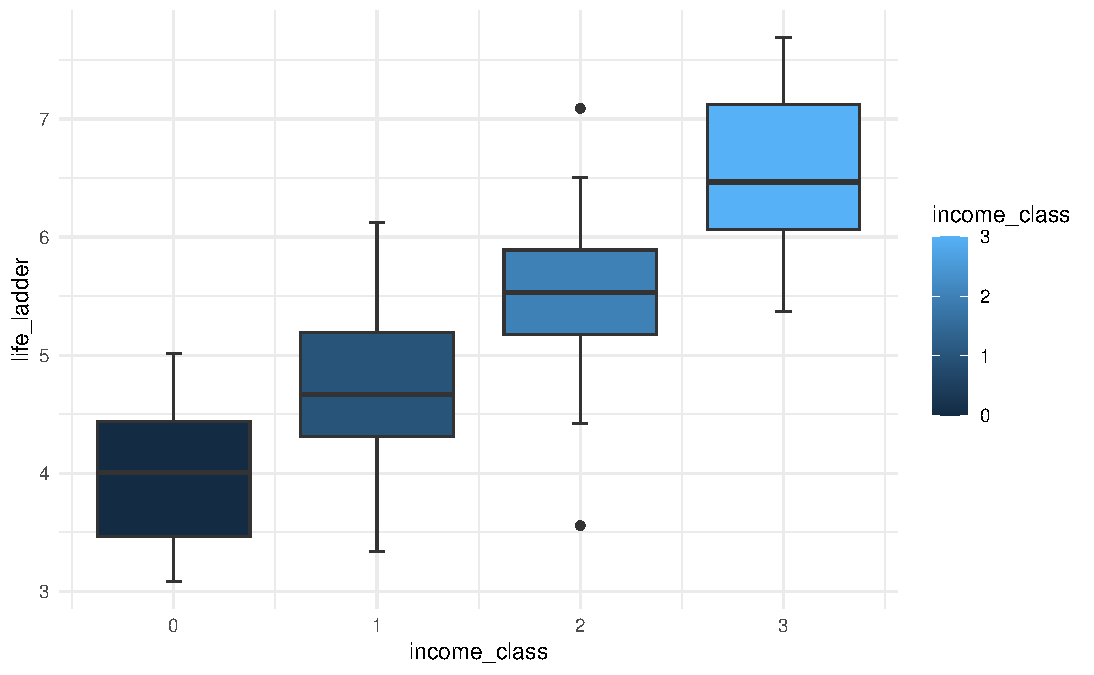
\includegraphics[width=1\textwidth]{figures/income_life.pdf}
    \label{fig:income_life}
\end{figure}

\newpage

\subsection{Propuesta metodológica}
La metodología escogida para llevar a cabo la tarea que se tiene puede dividirse en dos partes: \textit{el Coeficiente de correlación lineal de Pearson} y \textit{}{el Método Delta}. A continuación se procede a enunciar cada uno de ellos.

\begin{enumerate}
    \item \textbf{Coeficiente de correlación lineal de Pearson} \\
    
    El coeficiente de correlación de Pearson es un índice que mide el grado de variación entre distintas variables relacionadas linealmente. \\
    
    Supongamos que se tienen dos variables $X$, $Y$.
    Se define el coeficiente de correlación de Pearson entre estas dos variables como $r_{xy}$, con ello resulta que:
    
    \begin{equation*}
        -1 \leq r_{xy} \leq 1
    \end{equation*}
    
    Es importante mencionar que la magnitud de la relación vienen especificada por el valor numérico del coeficiente, mientras que el signo refleja la dirección de tal valor. Esto quiere decir que una relación de $+1$ es igual de fuerte a una relación $-1$, solamente cambia el sentido de esta. \\
    
    Una correlación positiva entre dos variables indica que a medida que una de ellas aumenta, la otra también lo hace. En el caso de que ambas aumenten en igual medida, se dice que son perfectamente positivas. De manera similar, una correlación negativa entre dos variables indica que a medida que una de ellas aumenta, la otra disminuye. En el caso de que ambas cambien en igual magnitud, se dice que son perfectamente negativas.\\
    
    El coeficiente de Pearson viene dado por la siguiente fórmula: \footnote{\cite{coef_pearsen}}
    
    \begin{equation}
        r_{xy} = \frac{\sum Z_x Z_y}{N} 
    \end{equation}
   
    Donde: 
   
    \begin{itemize}
        \item $Z_x$ es la desviación estándar de X
        \item $Z_y$ es la desviación estándar de Y
        \item N es la cantidad de datos 
    \end{itemize}

\pagebreak

\begin{lstlisting}[caption={Pruebas sobre el coeficiente de correlación lineal de Pearson}, label=lst:rchunk1]
# Para obtener una visualizacion de data en ggplot2 mas eficiente
install.packages("ggpubr")
library("ggpubr")

# Obtenemos la correlacion utilizando distintos metodos, en este caso Pearson, Kendall y Spearman, vamos a concentrarnos en Pearson, pero los otros metodos nos permite tener una idea mas clara del comportamiento de los datos.
cor(x, y, method = c("pearson", "kendall", "spearman"))
cor.test(x, y, method=c("pearson", "kendall", "spearman"))

# Grafico de dispersion de la correlacion
ggscatter(Data_relevante, x = "life_ladder", y = "log_gdp_per_capita", 
          add = "reg.line", conf.int = TRUE, 
          cor.coef = TRUE, cor.method = "pearson",
          xlab = "Miles/(US) gallon", ylab = "Weight (1000 lbs)")

# Prueba de normalidad Shapiro-Wilk de las variables
shapiro.test(Data_relevante$life_ladder) 
shapiro.test(Data_relevante$log_gdp_per_capita)

# Finalmente test de correlacion de Pearson
res <- cor.test(Data_relevante$log_gdp_per_capita, Data_relevante$life_ladder, method = "pearson")

# Interpretacion de resultados
# p.value: Valor p de la prueba
# estimate: coeficiente de correlacion
res
res$p.value
res$estimate

# Inspeccion grafica de la normalidad de las variables
ggqqplot(Data_relevante$life_ladder, ylab = "life_ladder")
ggqqplot(Data_relevante$log_gdp_per_capita, ylab = "log_gdp_per_capita")

# Se mostraran los graficos a continuacion
\end{lstlisting}
\newpage

\begin{figure}[!ht]
    \centering
    \caption{Gráfico de normalidad de life\_ladder}
    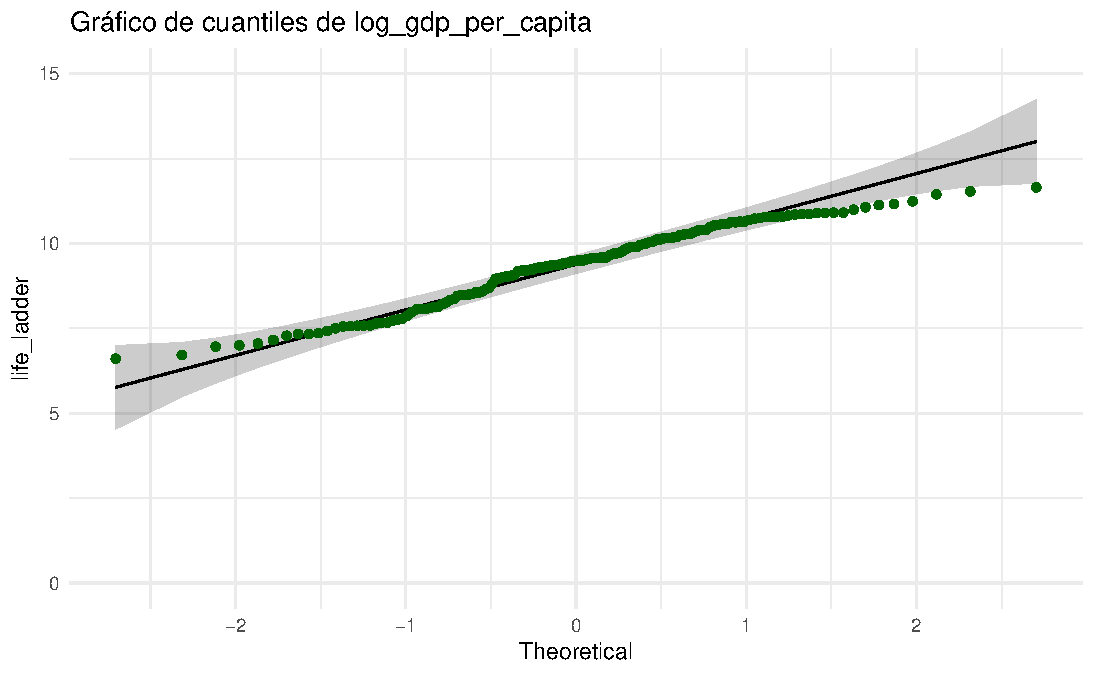
\includegraphics[width=0.8\textwidth]{figures/qqp_lgdp.pdf}
    \label{fig:correlaciones2}
\end{figure}

\begin{figure}[!ht]
    \centering
    \caption{Gráfico de normalidad de log\_gdp\_per\_capita}
    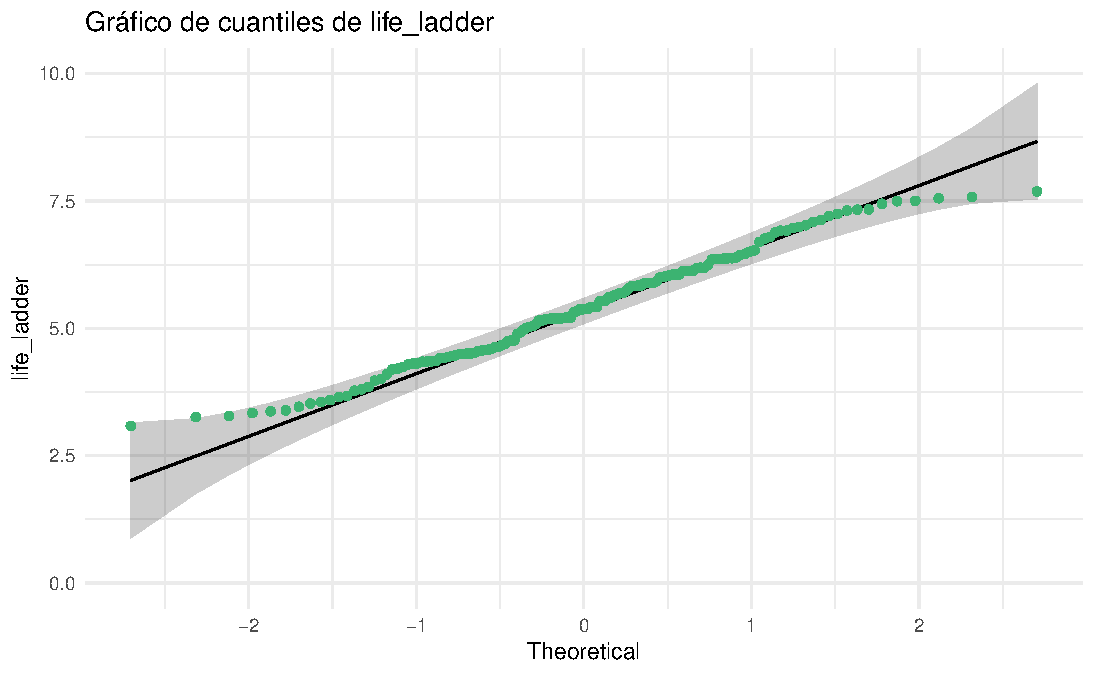
\includegraphics[width=0.8\textwidth]{figures/qqp_life.pdf}
    \label{fig:correlaciones3}
\end{figure}

\newpage
    \item \textbf{Método Delta} \\
    
    En el punto anterior, se detalló como obtener el coeficiente de correlación Pearson. Ahora bien, bajo el contexto del curso resulta fácil ver que esta medida puede tomarse como un estadístico, ya que este contiene todos los datos de las variables $X$ y $Y$. \\

    A su vez, dado que el procedimiento anterior se realizará con varias variables, podemos decir que obtendremos una serie de estadísticos, esto será de vital importancia para poder utilizar el Método Delta.\\

    Ahora bien, supongamos que se tiene un estimador $T_n$ para el parámetro $\theta$. Pero, nos interesa la cantidad $g(\theta)$ para alguna función $g$. Resulta natural pensar que $g(T_n)$ es un estimador natural.\\

    Justamente de esto trata el Método Delta, el cual se enuncia a continuación:

    \begin{mybox}{Teorema: Método Delta}
        Sea $T_n$ una sucesión de estadísticos tales que:
        
        \begin{equation*}
            \sqrt{n}(T_n - \theta) \xrightarrow[]{d} N(0, \sigma^2(\theta))
        \end{equation*}
        
        Sea $g: \mathbb{R} \longrightarrow \mathbb{R} \text{ diferenciable en } \theta \text{ con } g'(\theta) \neq 0$. 
        Entonces: 

        \begin{equation*}
            \sqrt{n}[g(T_n) - g(\theta)] \xrightarrow[]{d} N(0, [g'(\theta)^2]\sigma^2(\theta))
        \end{equation*}

        \flushright\cite{asymptotic_stats}
    \end{mybox}

    Una vez mencionado el teorema, lo que se buscará con él será aproximar la distribución de nuestra variable, por medio de los estadísticos obtenidos al realizar la correlación. 
\pagebreak

\begin{lstlisting}[caption={Estimación de la distribución utilizando el método delta}, label=lst:rchunk2 ] 
# Obtenemos la variable de estudio
X <- Data_relevante$life_ladder

# Se calcula el promedio y la varianza de la variable de estudio
prom_X <- mean(X)
var_X <- var(X)

# Se define una funcion dependiente de la variable de estudio Y = 2X + 3
Y <- function(x) 2*x + 3

# Se calcula la derivada de Y con la media de X
Y_prima <- function(x) 2

# Se aplica el metodo delta para estimar la varianza de Y
var_Y <- (Y_prima(prom_X))^2 * var_X

# Se asume que Y sigue una distribucion normal, se determina su promedio y desviacion estandar
mean_Y <- Y(prom_X)
sd_Y <- sqrt(var_Y)
\end{lstlisting}

\end{enumerate}

\textbf{Nota:} Este es el primer acercamiento que se tiene con el modelo delta, se espera perfeccionarlo para las siguientes entregas, esto con ayuda del profesor y las fuentes dadas por el mismo.
\newpage

\subsection{Construcción de fichas de resultados}

\begin{table}[H]
    \caption{Ficha de Resultados 1}
    \begin{center}
        \begin{tabular}{  m{3cm} | m{12cm}  }
        \hline\textbf{ Encabezado} & \textbf{Contenido }\\ \hline
        Nombre de su hallazgo/resultado: &  Correlación Positiva de las variables de interés.\\ \hline
        Resumen en una oración: &  Se pudo encontrar una relación positiva de las variables que queríamos utilizar como factores con el índice de felicidad. 
\\ \hline
        Principal característica: &  Ahora que sabemos que existe esta correlación dado el análisis que realizamos, entonces podemos reforzar esta idea usando más material bibliográfico.\\ \hline
        Problemas o posibles desafíos: &  Cabe la posibilidad de utilizar un método incorrecto para encontrar la correlación o que pase que correlación no implica causalidad, entonces hay que tener especial cuidado con como interpretamos los datos y si la correlación en realidad tiene sentido o no. \\ \hline
        Resumen en un párrafo: & Se utilizó una matriz de correlación para verificar qué variables presentaban una correlación, aunque este análisis se hizo para todas las variables, las que son de nuestro interés, son sólo las 5 mencionadas anteriormente. Se realizó una limpieza de la base de datos para tener unos datos depurados y que no vayan a ensuciar el análisis, también hubieron países que no aportaron ciertos datos, esto pudo haber afectado al análisis de éstos. \\ \hline
        \end{tabular}
    \end{center}
\end{table}

\begin{table}[H]
    \caption{Ficha de Resultados 2}
    \begin{center}
        \begin{tabular}{  m{3cm} | m{12cm}  }
        \hline\textbf{ Encabezado} & \textbf{Contenido }\\ \hline
        Nombre de su hallazgo/resultado: &  Correlación entre corrupción y polución del aire\\ \hline
        Resumen en una oración: &  A partir del análisis de datos, se observó una relación positiva  entre la polución del aire y el índice de corrupción en la base de datos.
\\ \hline
        Principal característica: &  No se esperaba encontrar una correlación positiva entre la corrupción y ninguna variable del modelo, pues se interpreta la corrupción como un concepto de perjuicio en la sociedad. Sin embargo, a partir del análisis pudimos determinar que hay una correlación positiva.\\ \hline
        Problemas o posibles desafíos: &  Hay algo importante que mencionar, y es que correlación no implica causalidad, así que habría que buscar material que apoye específicamente este resultado, para determinar si el análisis de esta variable es o no de importancia. \\ \hline
        Resumen en un párrafo: & Para encontrar este hallazgo se utilizó la matriz de correlación, una hipótesis de este resultado es que al haber corrupción en los gobiernos, las personas encargadas de llevar a cabo la utilización de fondos, podrían no estar utilizando los fondos para lo que deberían ser utilizados, como protección ambiental, por ejemplo. Se podría proponer buscar más información de esta correlación, para determinar si hay o no una relación real, en la tercera bitácora. \\ \hline
        \end{tabular}
    \end{center}
\end{table}

\begin{table}[H]
    \caption{Ficha de Resultados 3}
    \begin{center}
        \begin{tabular}{  m{3cm} | m{12cm}  }
        \hline\textbf{ Encabezado} & \textbf{Contenido }\\ \hline
        Nombre de su hallazgo/resultado: &  Correlación entre Producto Interno Bruto per Capita y el Índice de Percepción de la Corrupción\\ \hline
        Resumen en una oración: &  A partir del análisis de datos, se observó una relación positiva  entre el Producto Interno Bruto y el Índice de Corrupción en la base de datos.
\\ \hline
        Principal característica: &  A partir del análisis de datos se encontró la existencia de una relación positiva entre las dos variables, lo que muestra que a medida que un país tienen un mayor producto interno bruto per capita también presenta un alto índice de percepción de la corrupción.\\ \hline
        Problemas o posibles desafíos: &  Hay algo importante que mencionar, y es que correlación no implica causalidad, así que resulta sensato investigar fuentes fiables que expliquen si existe una relación teórica entre un alto grado de corrupción en relación a un producto interno bruto per capita mayor. \\ \hline
        Resumen en un párrafo: & Para encontrar este hallazgo se utilizó la matriz de correlación, una hipótesis de este resultado podría basarse en el hecho de que un país con un mayor producto interno bruto per capita resulta mas tentador para los gobiernos a dedicarse a actividades éticamente cuestionables con respecto al manejo de finanzas publicas. \\ \hline
        \end{tabular}
    \end{center}
\end{table}

\begin{table}[H]
    \caption{Ficha de Resultados 4}
    \begin{center}
        \begin{tabular}{  m{3cm} | m{12cm}  }
        \hline\textbf{ Encabezado} & \textbf{Contenido }\\ \hline
        Nombre de su hallazgo/resultado: &  Correlación entre clase social y esperanza de vida\\ \hline
        Resumen en una oración: &  A partir del análisis de datos, se observó una relación positiva  entre una alta clase social y la esperanza de vida en la base de datos.
\\ \hline
        Principal característica: &  A partir del análisis de datos se encontró la existencia de una relación positiva entre las dos variables, lo que muestra que a medida que un país presenta una clase social dominante de un estrato más alto tiene a su vez una mayor esperanza de vida.\\ \hline
        Problemas o posibles desafíos: &  Al tratarse la clase social de una variable categórica, las separaciones que existen entre distintos países con la forma en la estructuran su clase dominante no es estandarizada, por lo que pueden existir sesgos. \\ \hline
        Resumen en un párrafo: & Para encontrar este hallazgo se utilizó la matriz de correlación, una clase social dominante de un estrato más alto, va a tener un acceso mas facilitado a servicios de una mayor calidad, incluyendo los de salud, lo cual esta demostrado mediante estudios anteriores que influye de forma positiva en la esperanza de vida. \\ \hline
        \end{tabular}
    \end{center}
\end{table}

\begin{table}[H]
    \caption{Ficha de Resultados 5}
    \begin{center}
        \begin{tabular}{  m{3cm} | m{12cm}  }
        \hline\textbf{ Encabezado} & \textbf{Contenido }\\ \hline
        Nombre de su hallazgo/resultado: &  Correlación entre Índice de Felicidad y Log del Producto Interno Bruto\\ \hline
        Resumen en una oración: &  A partir del gráfico de dispersión, se observó una relación positiva  entre el Índice de Felicidad y el Log del Producto Interno Bruto. \\ \hline
        Principal característica: &  A partir del análisis de datos se encontró la existencia de una relación positiva entre las dos variables, lo que se muestra de forma positiva con la literatura que se ha desarrollado, que denota una relación positiva entre la Felicidad y variables económicas, siendo el Producto Interno Bruto la más importante de estas.\\ \hline
        Problemas o posibles desafíos: &  La Felicidad se observa como una variable compleja para la cual no resulta completamente adecuado realizar un análisis enfocado únicamente en el área económica, sino que presente elementos psicológicos y sociológicos \\ \hline
        Resumen en un párrafo: & Para encontrar este hallazgo se utilizó tanto la matriz de correlación como el gráfico de dispersión, valores de magnitudes cada vez mayores están relacionados con un mayor Índice de Felicidad según la literatura que se abarca en el estudio presente. \\ \hline
        \end{tabular}
    \end{center}
\end{table}
